% meta.concepts: 2D moments
% meta.tags: realistic
% acknowledge: Engineering Statics: Open and Interactive
% source: Exercise 4.9 of online edition

Force $\bar{F}$, which has a magnitude of 4 kN, acts along a line passing through points $D$ and $D^\prime$.   The grid units are in $m$ and counter-clockwise moments are positive.  Determine the moment of the force about points $A$, and $B$ using the definition of the moment: $M = F \cdot d_{\perp}$.

\begin{enumerate}
  \item Find the length of the line segment from A to D (or any other point on the line of action of $\bar{F}$).
  \begin{itemize}\item $d = $\end{itemize}
  \item Find the angle ($<= 90^\circ$) between segment $\bar{AD}$ and the line of action of $\bar{F}$.
  \begin{itemize}\item$\theta_A = $\end{itemize}
  \item Find the perpendicular distance between point $A$ and the line of action of force $\bar{F}$.
  \begin{itemize}\item$d_{\perp} = $ \end{itemize}
  \item Use the definition of a moment to computer $M_A$.
  \item In the same way, determine the moment of the force $\bar{F}$ about point $B$.
\end{enumerate}

\begin{figure}[ht!]
  \centering
  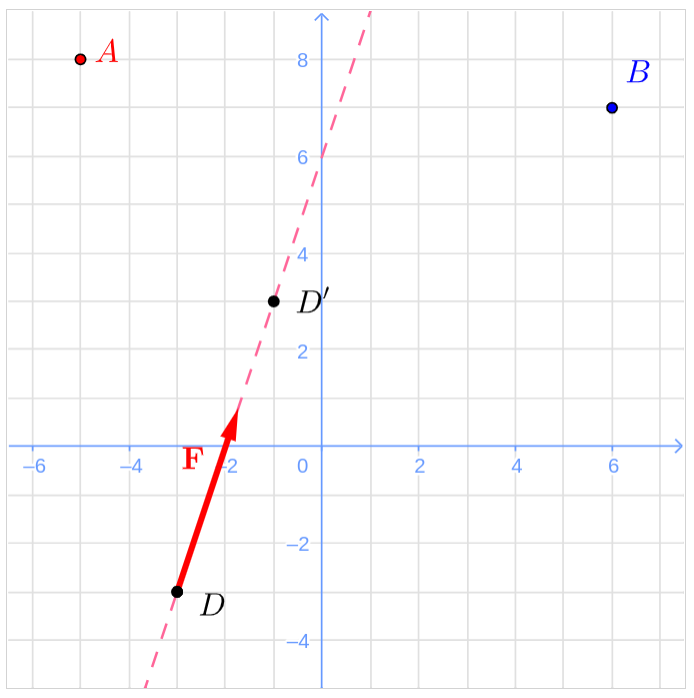
\includegraphics[width=0.8\textwidth,height=0.5\textheight,keepaspectratio]{fig.png}
\end{figure}

\iftoggle{flagSoln}{%
\vspace{.5cm}
\rule{\textwidth}{.4pt}
\vspace{.5cm}
\textbf{Solution:}
\begin{enumereate}
  \item $d = 11.18 m$
  \item $\theta_A = 28.74 ^\circ$
  \item $d_{\perp} = 5.376$
  \item $M_A = 21.5 m \cdot kN$
  \item $M_B = 21.5 m \cdot kN$
\end{enumerate}
}{%
}%
